\documentclass[11pt,notitlepage]{article}
\usepackage{graphicx}
\usepackage{amsmath}            % adds more math symbols
\usepackage{amssymb}
\usepackage{multicol}
\title{Neisseria Ortholog Analysis Tool}
\author{Leo Przybylski\\
\texttt{przybyls@arizona.edu}}

\newcommand{\question}[2]{\textbf{#1.} #2}
\newcommand{\subquestion}[2]{\par\hspace{0.5cm} \textbf{#1)} #2}
\newenvironment{answer}{\endpar%

}

    % Give wider margins; gives more text per page.

\setlength{\topmargin}{0.00in}
\setlength{\textheight}{8.75in}
\setlength{\textwidth}{6.625in}
\setlength{\oddsidemargin}{0.0in}
\setlength{\evensidemargin}{0.0in}

\setlength{\parindent}{0.0cm}	% Don't indent the paragraphs
%\setlength{\parskip}{0.4cm}	% distance between paragraphs

\begin{document}
  \maketitle
  \tableofcontents

  \abstract{\ldots
}
  {\setlength{\baselineskip}%
           {0.0\baselineskip}
  \section*{\hfill Background}
  \hrulefill \par}
  When a blast query is made, results are recorded with the identifier of the query
  as well as the identifier for the result or hit. The convention used to name the
  each query is a combination of gene and contig number. The records of blast output
  can be organized into several different types of meaningful information.


 %% \includegraphics[width=120mm]{api/images/sample-graph1.png}

  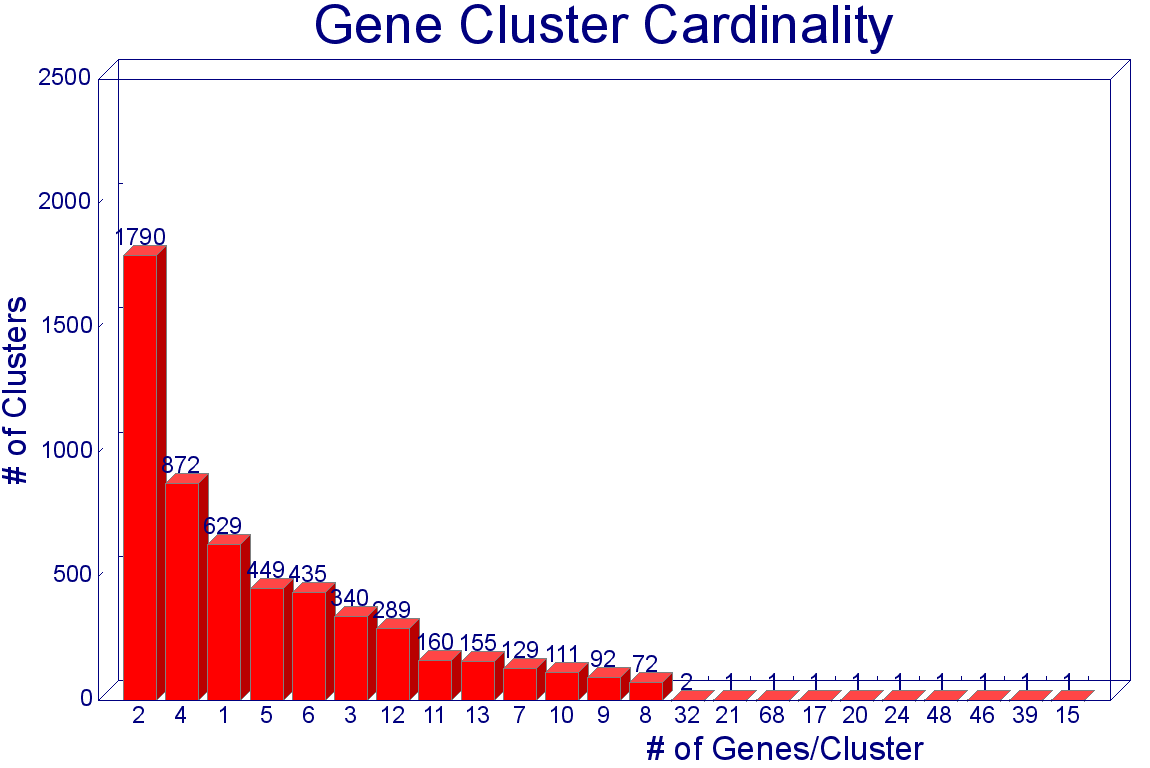
\includegraphics[width=145mm]{i90_a90_graph.png}


  One way in particular is to group records related by query and or hit information as
  clusters. We can then provide statistical information on clusters. By grouping clusters
  with the same cardinality of edges, we can analyze trends between different families
  of bacteria. One can analyze that similar families can grow at the same rate or that 
  similar families can recombine with similar genes. This is the benefit of ortholog
  analysis of gene clusters.

  {\setlength{\baselineskip}%
           {0.0\baselineskip}
  \section*{\hfill Clusters}
  \hrulefill \par}
  A Cluster is a set of edges where the query identifiers match. For example, in the
  following blast results:

  \noindent \verb|AP206_contig00001_4923-1612	cinerea_contig00013_10696-7277	47.65	1129	517	23	29	1103	31	1139	0.0	 884|

  \noindent \verb|AP206_contig00001_4923-1612	elongata_contig01464_47682-51131	46.11	1156	545	24	7	1103	13	1149	0.0	 851|
  \\

  The records belong in the same cluster because they were results of the same query. Not
  all records that match the query identifier become edges. 

  \subsection{Identifying Cluster Edges} 
  
  A gene may relate to another gene cluster by defining a cross-cluster relationship. For example, if we added the 
  following data:

  \noindent \verb|sicca_contig00265_4037-6052	AP206_contig00001_4923-1612	24.92	309	170	14	408	671	812	1103	4e-04	42.4|

  The above will create an edge between \emph{AP206\_contig00001\_4923\-1612} and \emph{sicca\_contig00265\_4037\-6052}
  clusters. Then, all of the hits relating to the \emph{sicca\_contig00265\_4037\-6052} query will
  suddenly be added to the cluster as well.

  The edge must also fulfill 
  identity percentage and alignment length ratio requirements. The identity percentage must
  be with in the bounds specified at runtime. The identity percentage requirement is within the range 
  $\in \{30, 45, 60, 75, 90\}$. Likewise, the alignment length ratio must be within the range
  $\in \{50, 70, 90\}$ which is defined at runtime. Again, the identity percentage and
  alignment length ratio requirements are variable and determined at runtime. This study
  provided results on each permutation of identity percentage and alignment length ratio.



  {\setlength{\baselineskip}%
           {0.0\baselineskip}
  \section*{\hfill Conclusion}
  \hrulefill \par}
  
  \subsection{Poisson Distributions}

  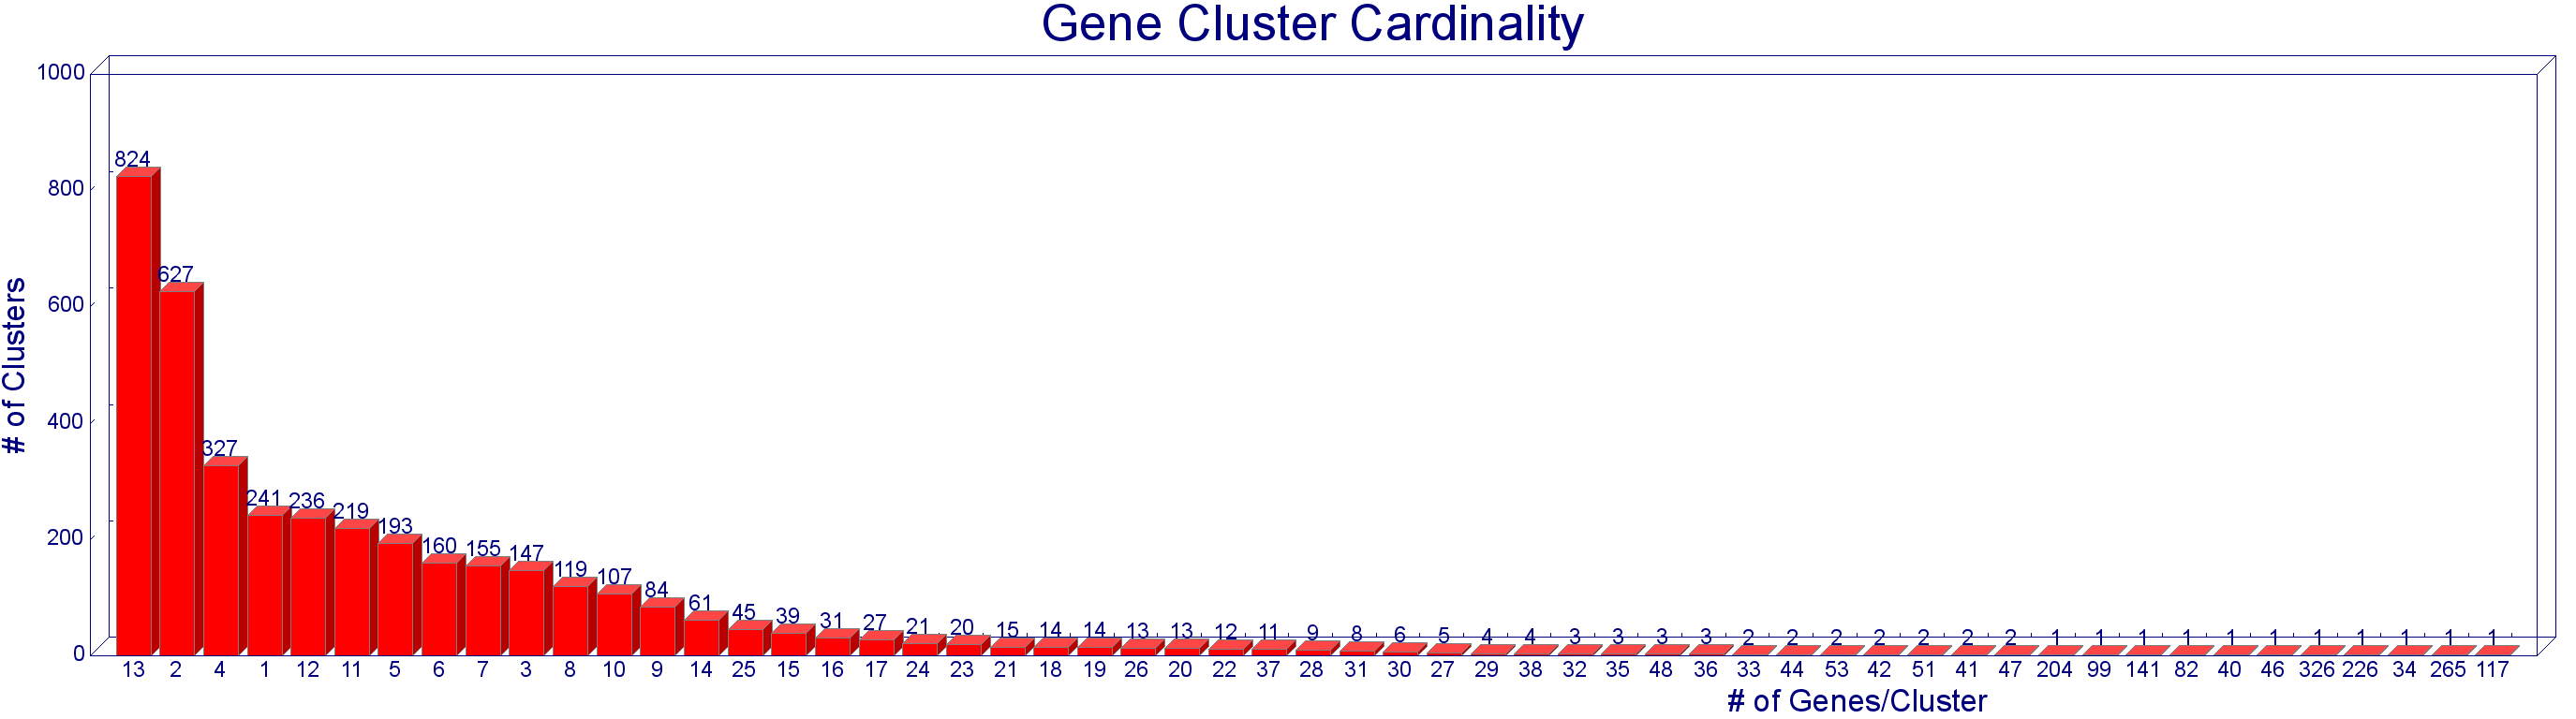
\includegraphics[width=145mm]{i30_a50_graph.png}
  
  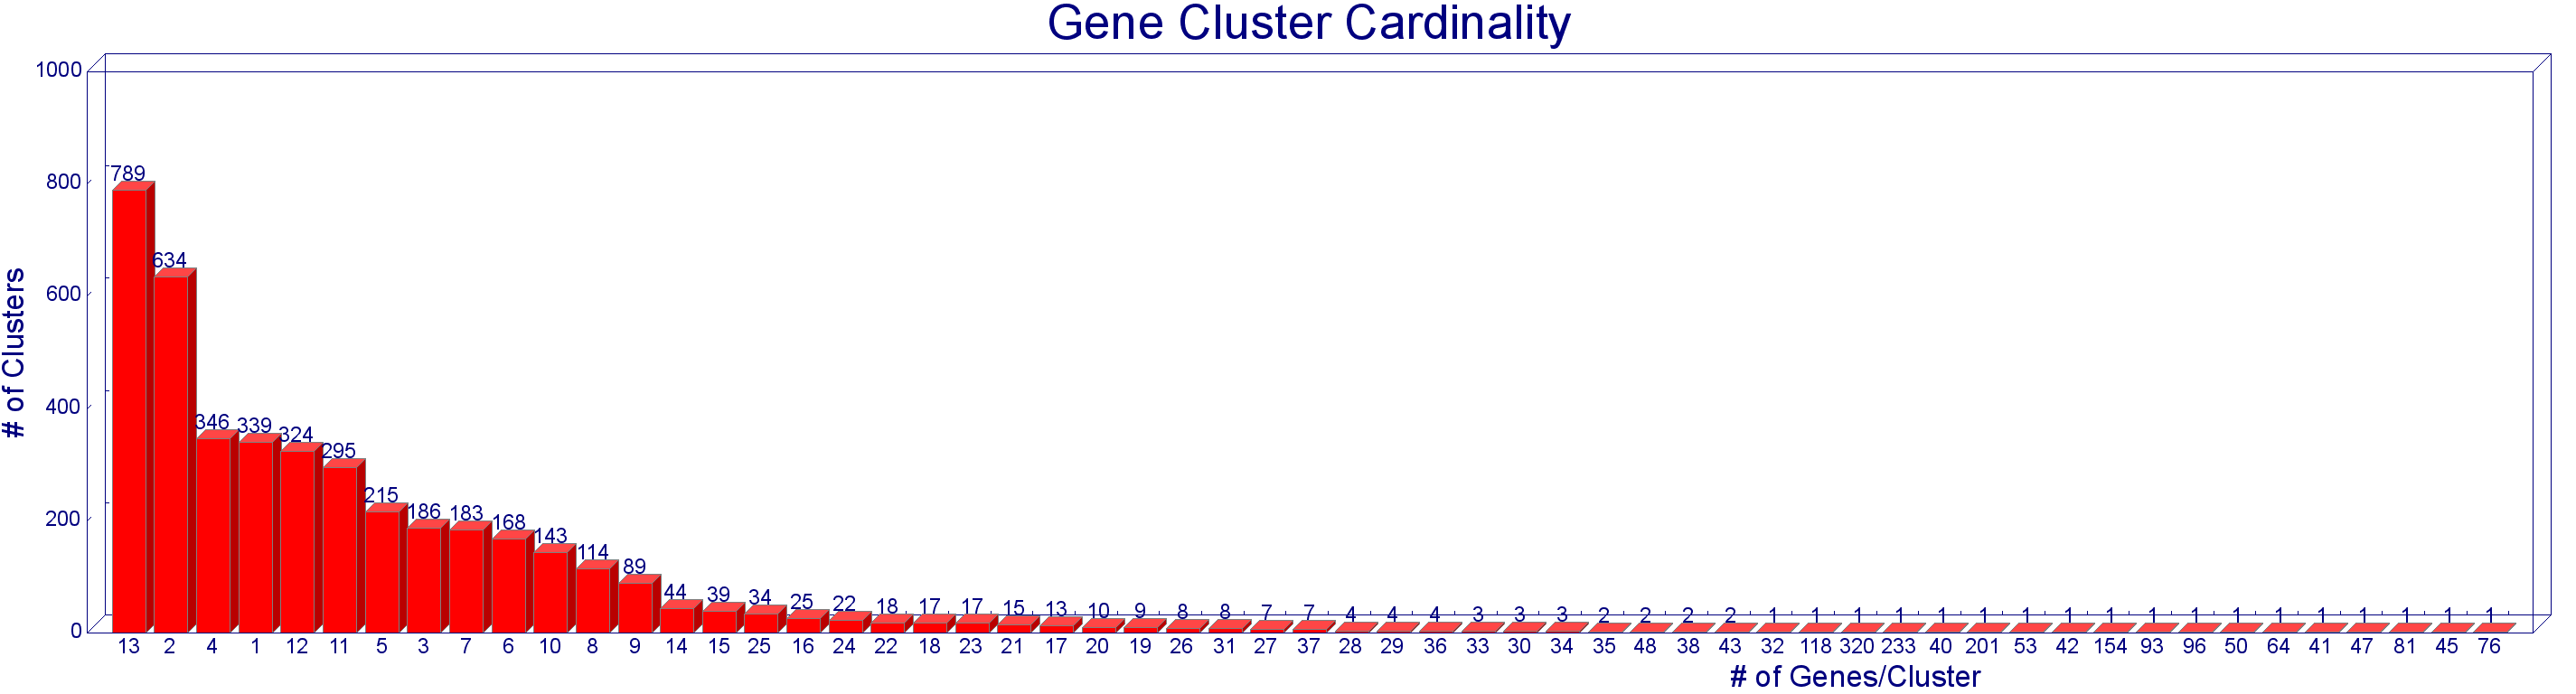
\includegraphics[width=145mm]{i30_a70_graph.png}
  
  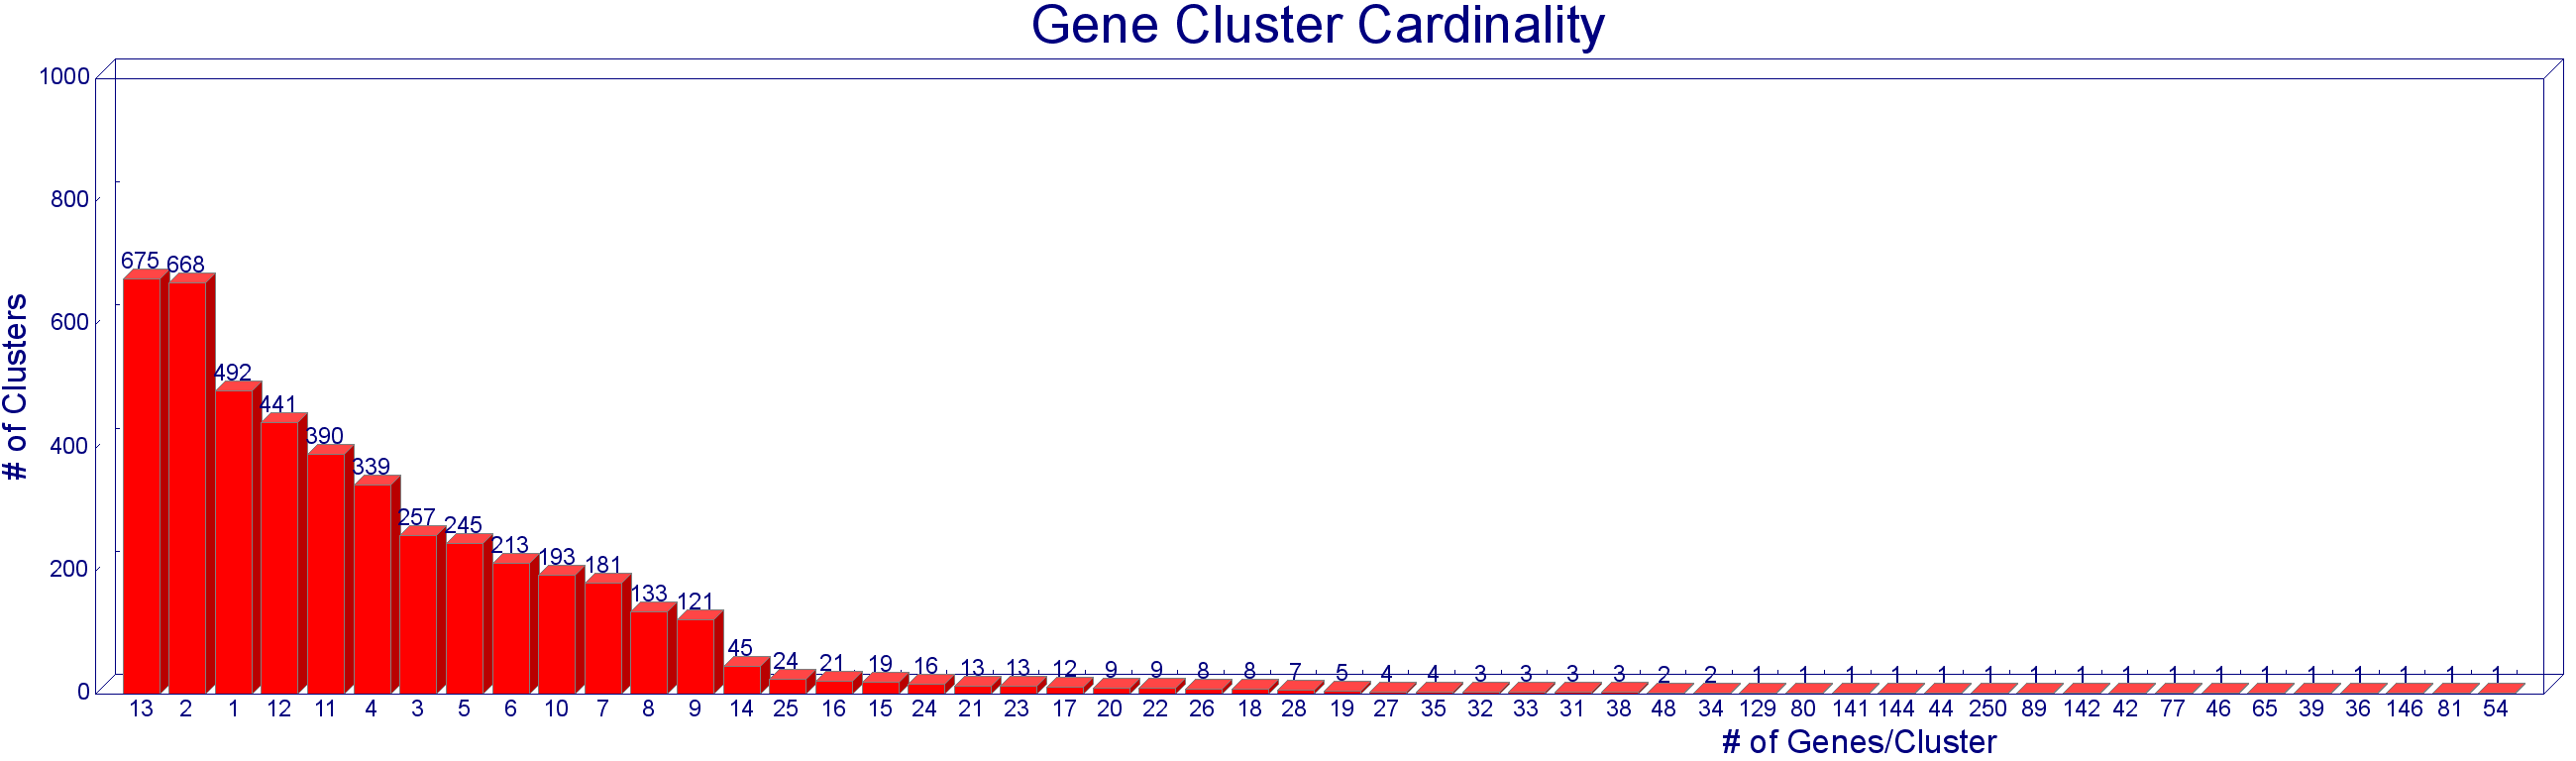
\includegraphics[width=145mm]{i30_a90_graph.png}
  
  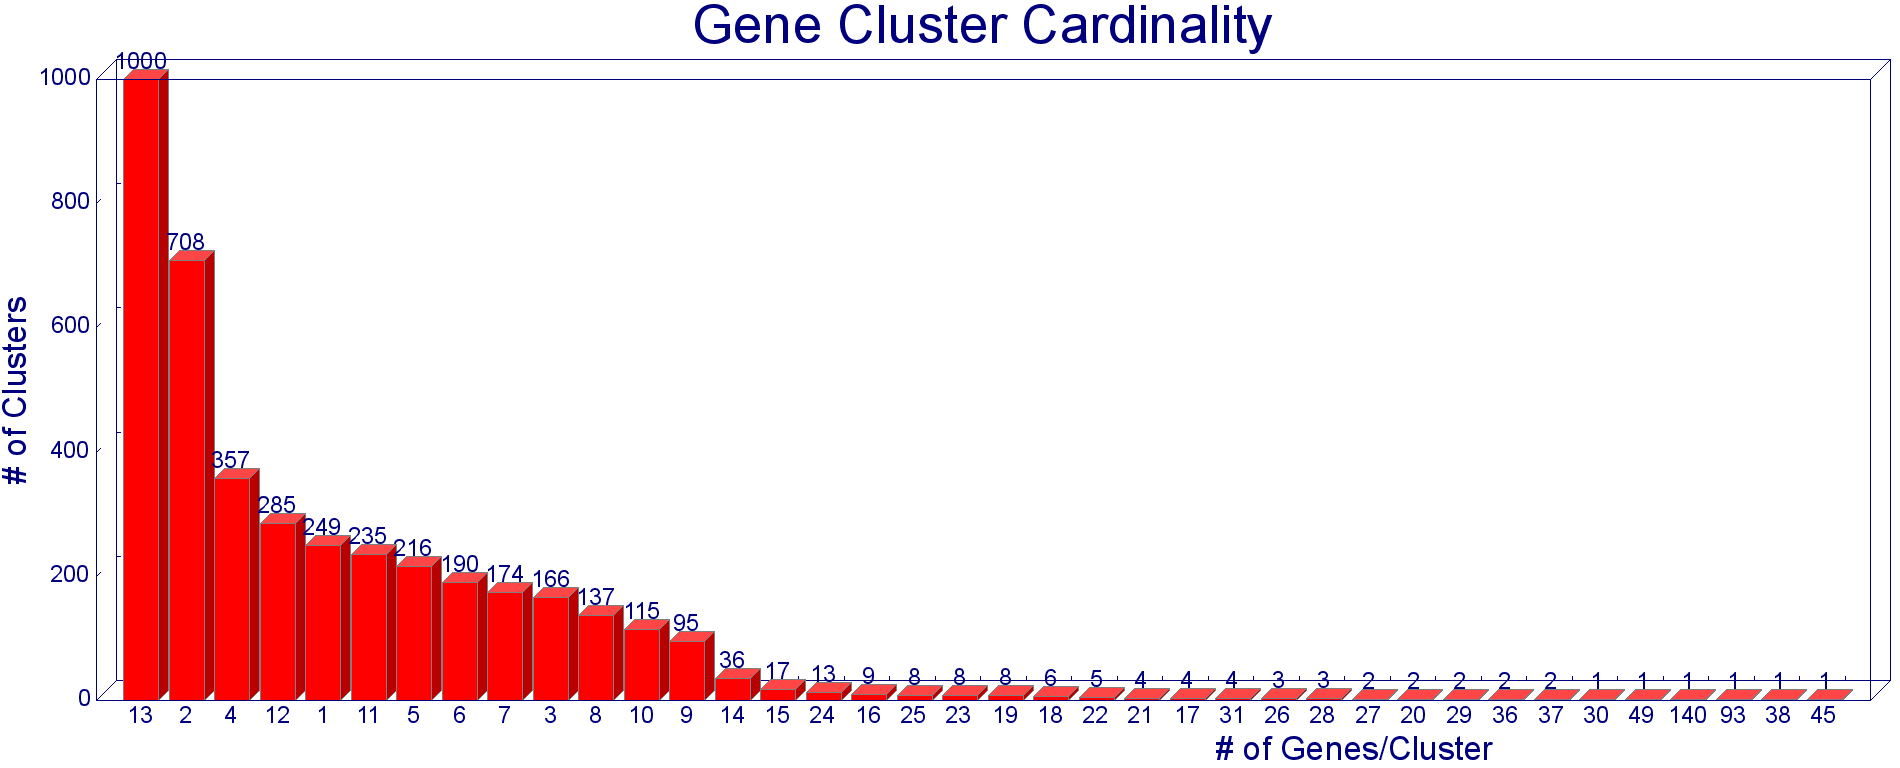
\includegraphics[width=145mm]{i45_a50_graph.png}
  
  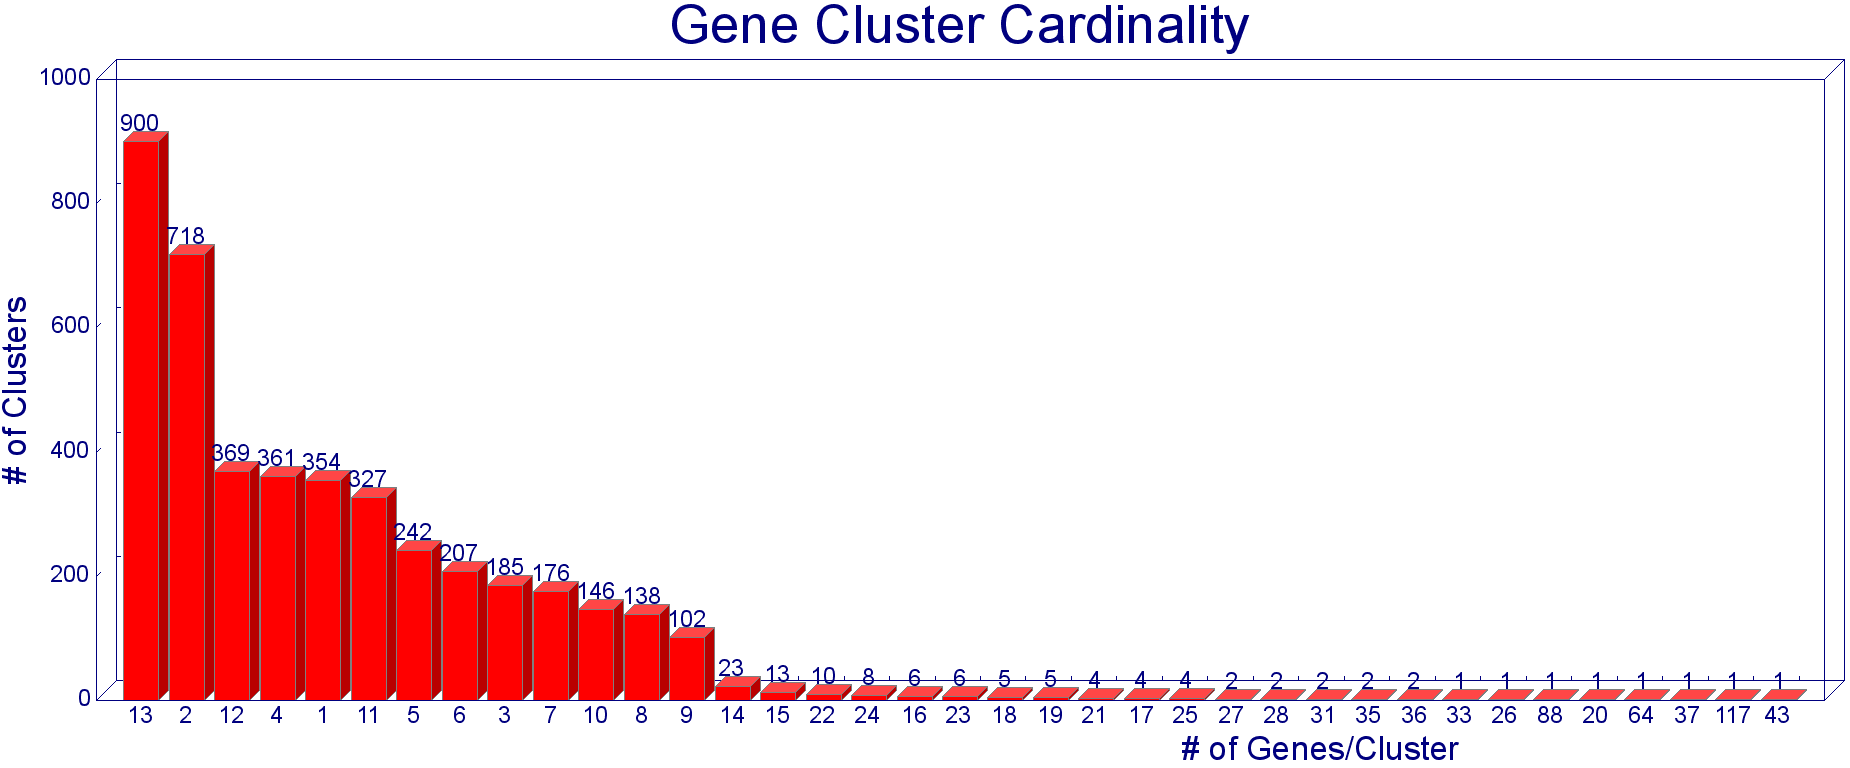
\includegraphics[width=145mm]{i45_a70_graph.png}
  
  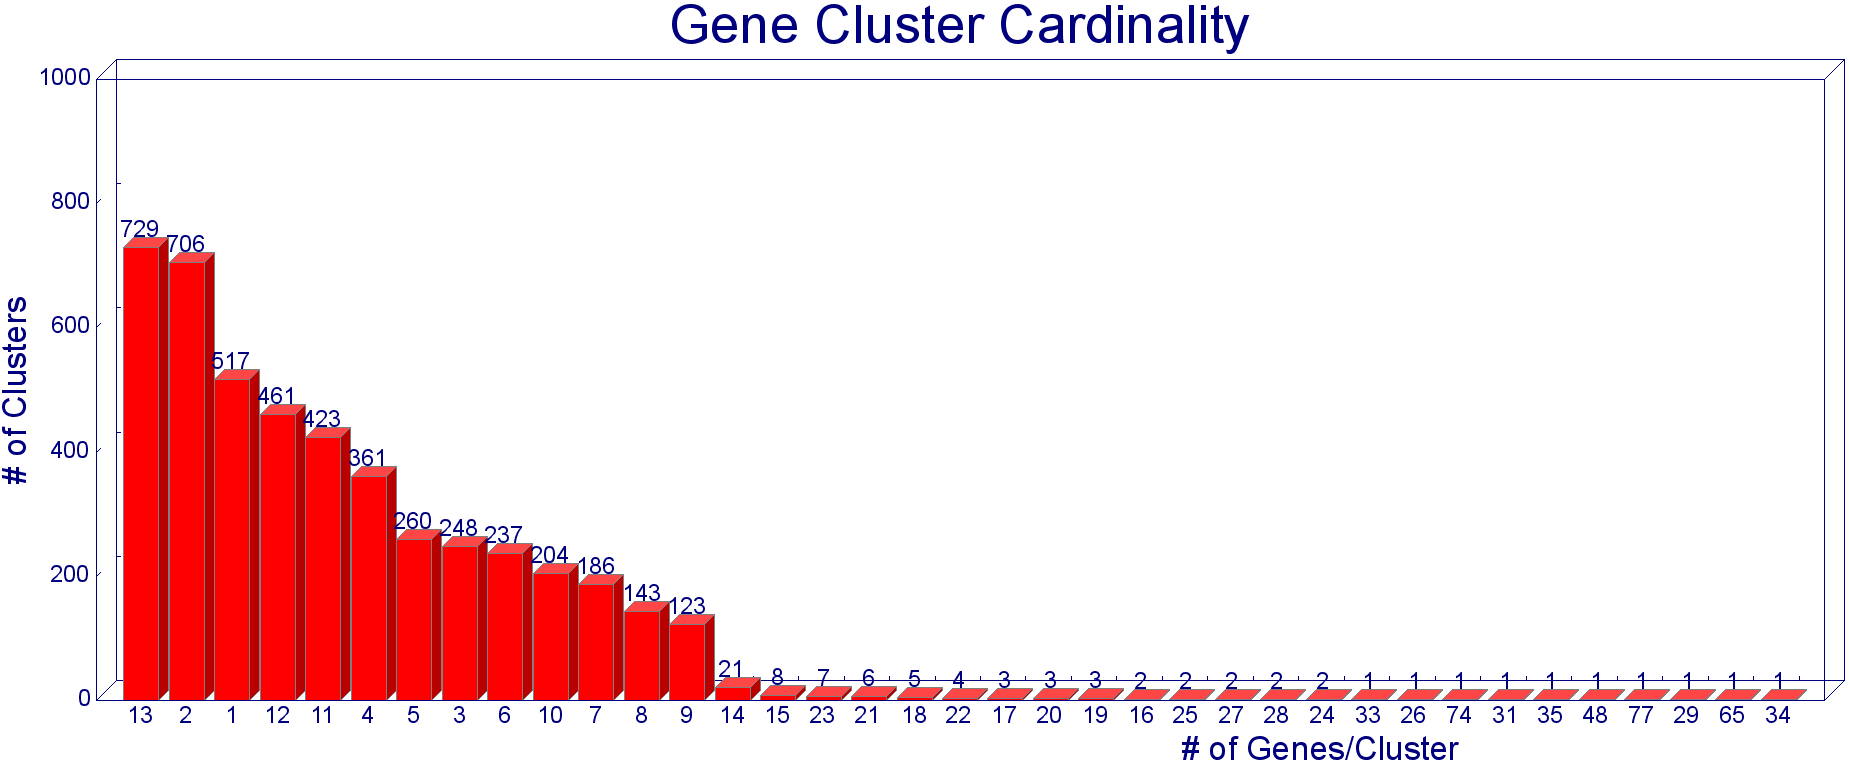
\includegraphics[width=145mm]{i45_a90_graph.png}
  
  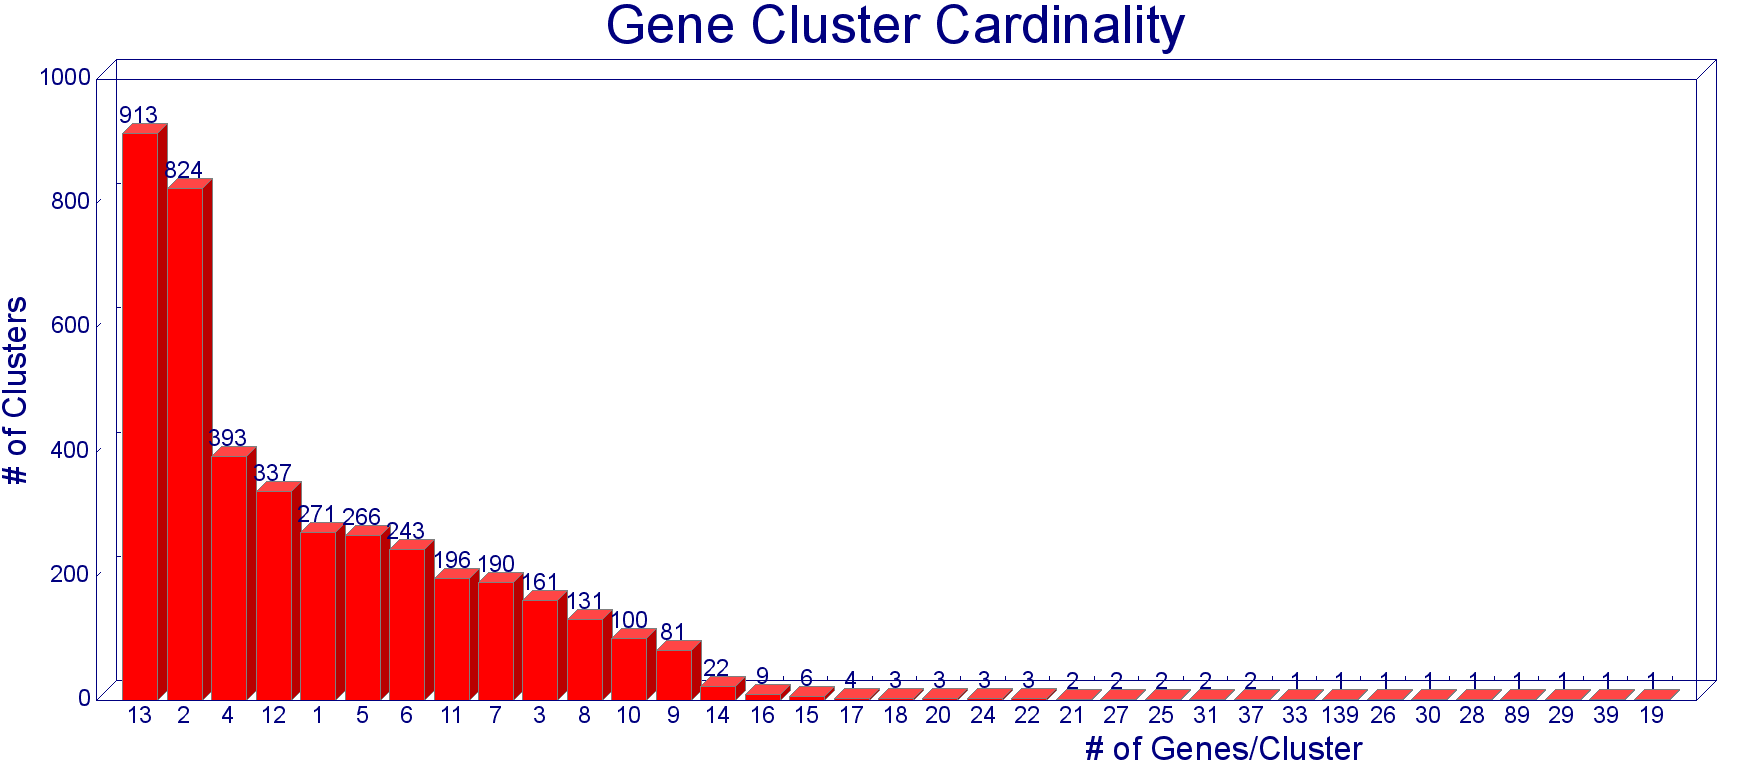
\includegraphics[width=145mm]{i60_a50_graph.png}
  
  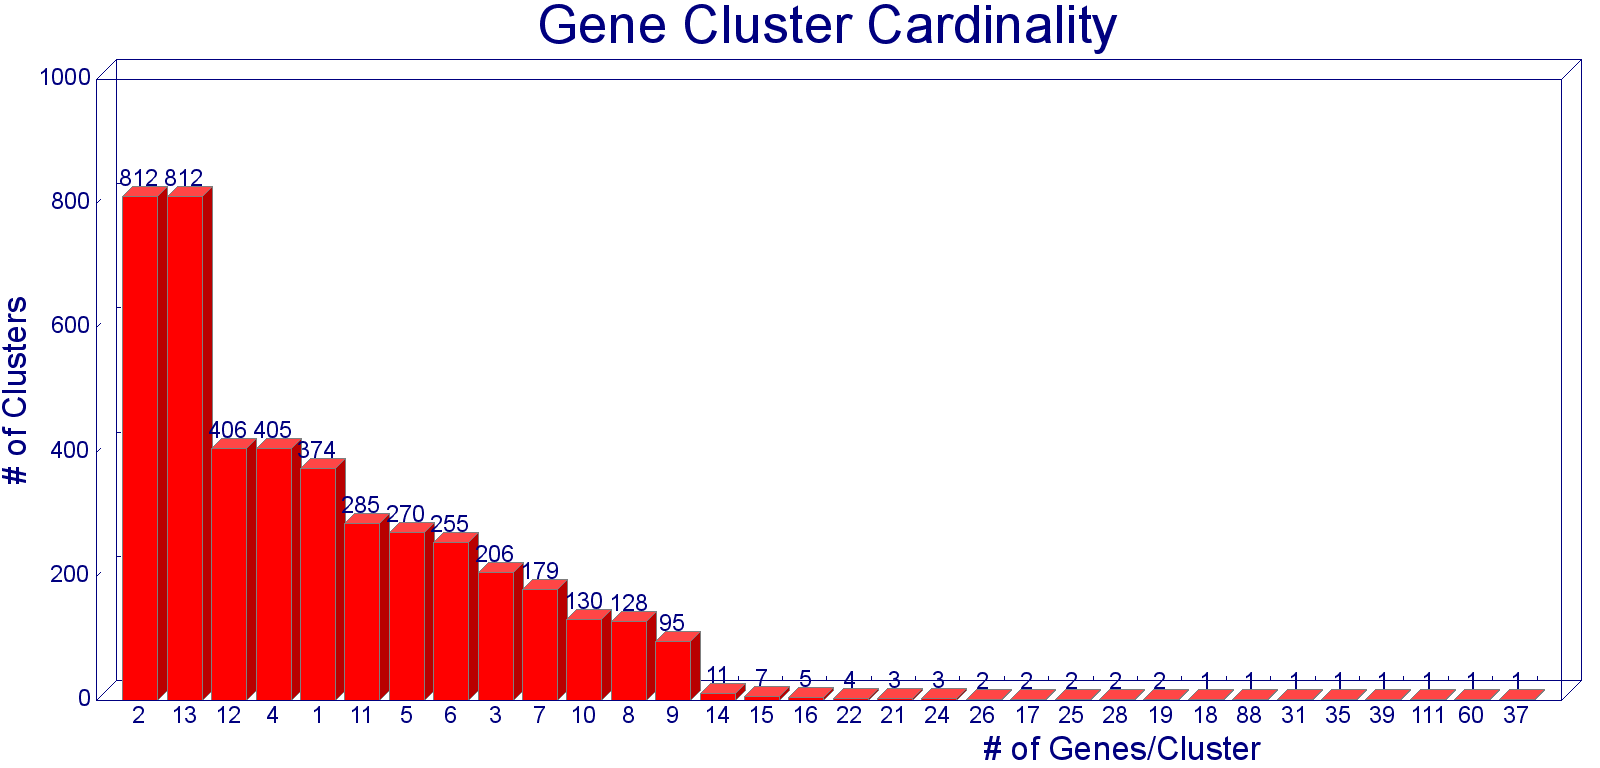
\includegraphics[width=145mm]{i60_a70_graph.png}
  
  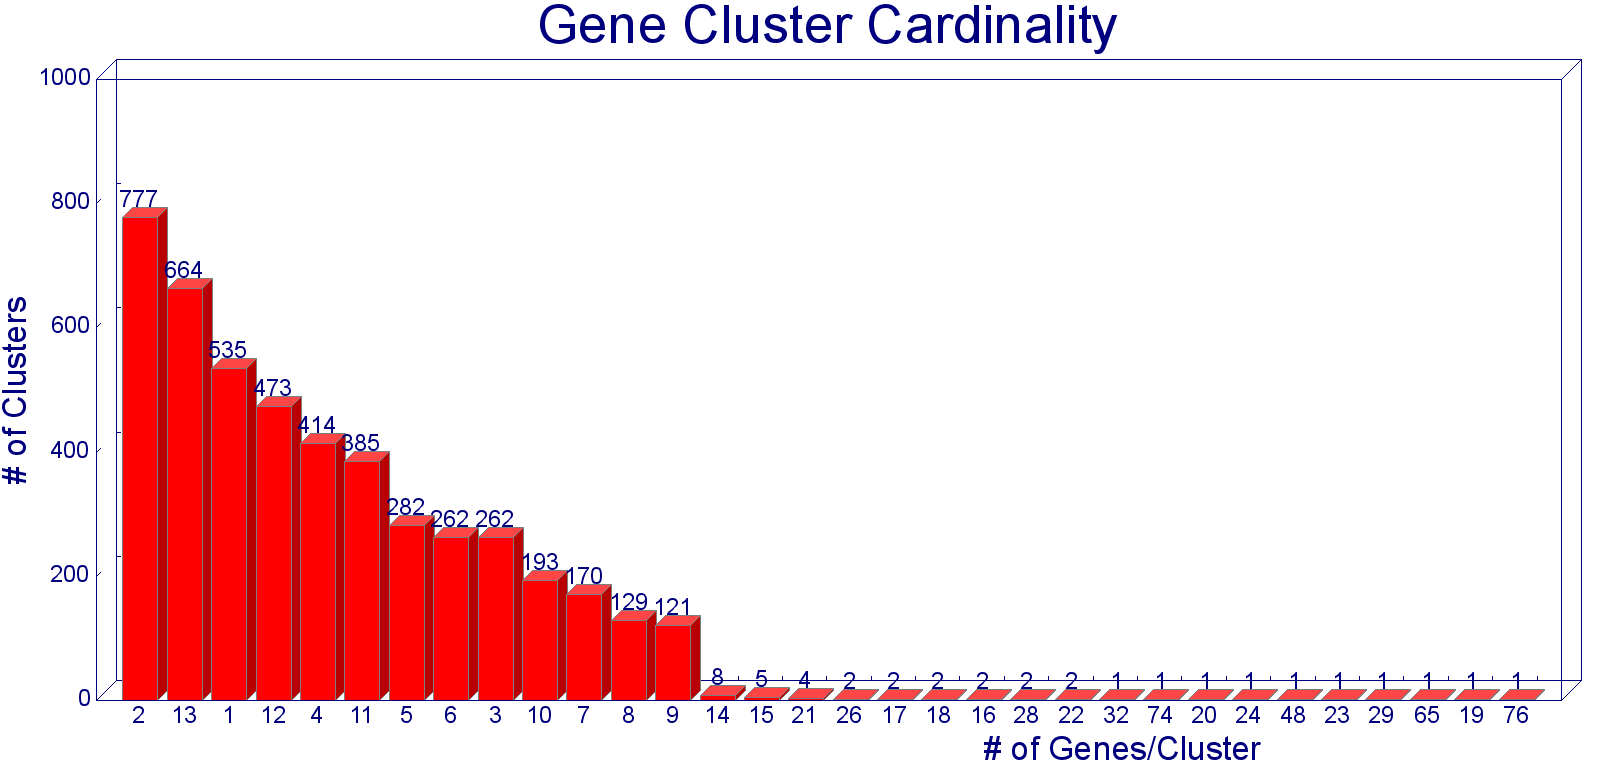
\includegraphics[width=145mm]{i60_a90_graph.png}
  
  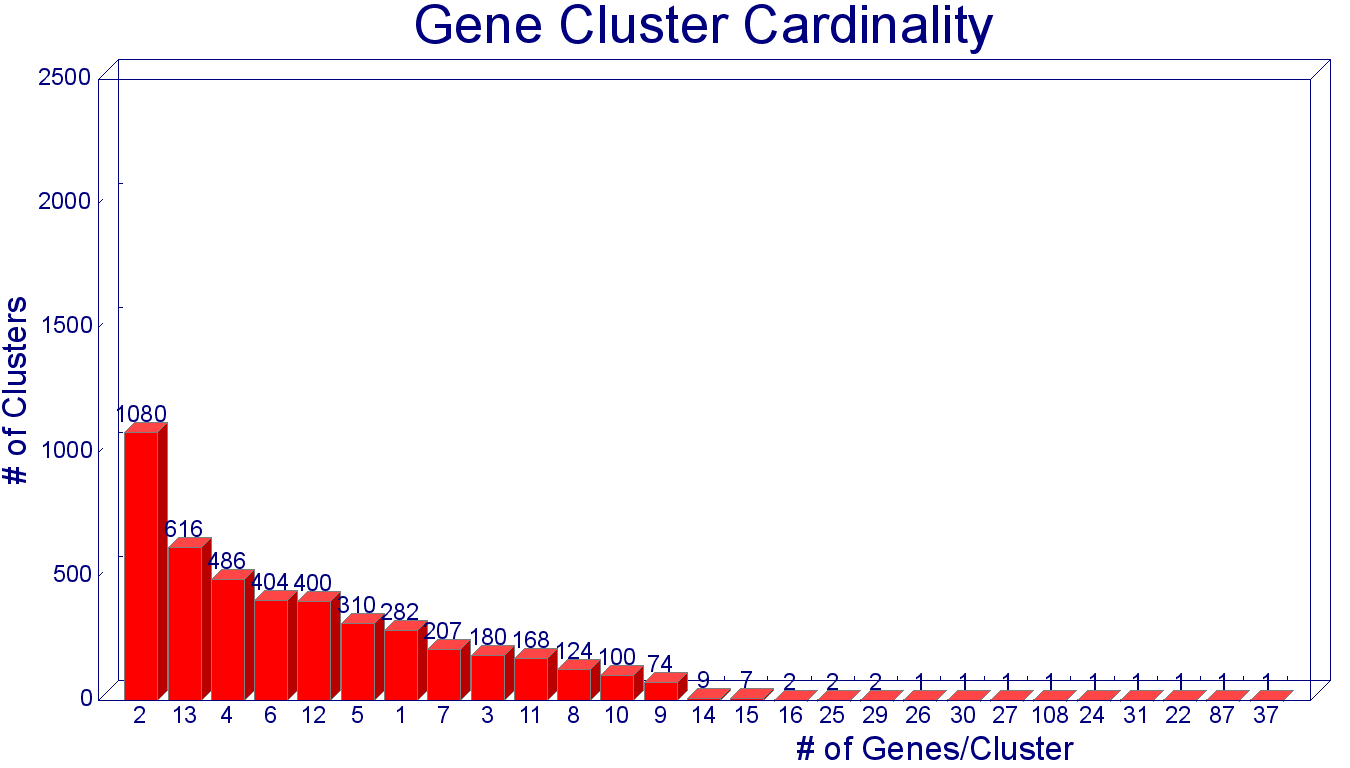
\includegraphics[width=145mm]{i75_a50_graph.png}
  
  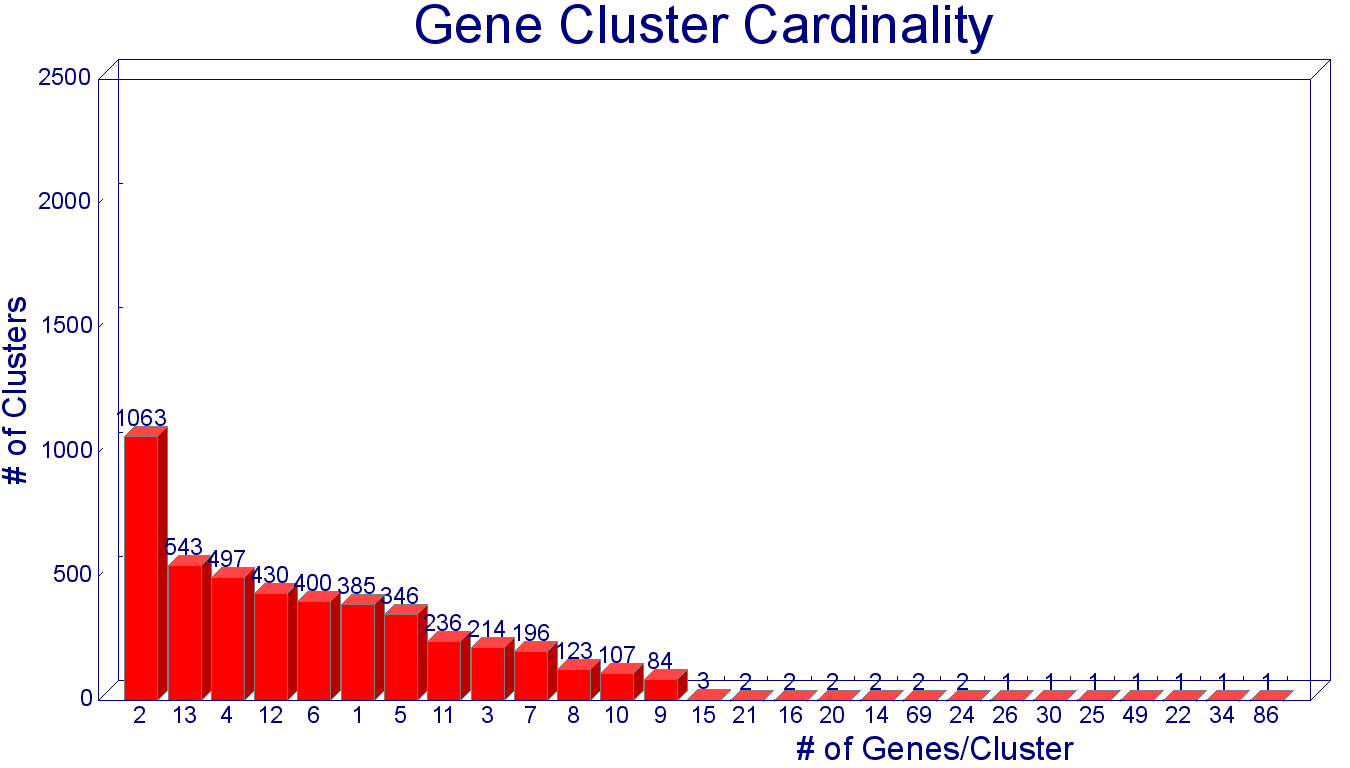
\includegraphics[width=145mm]{i75_a70_graph.png}
  
  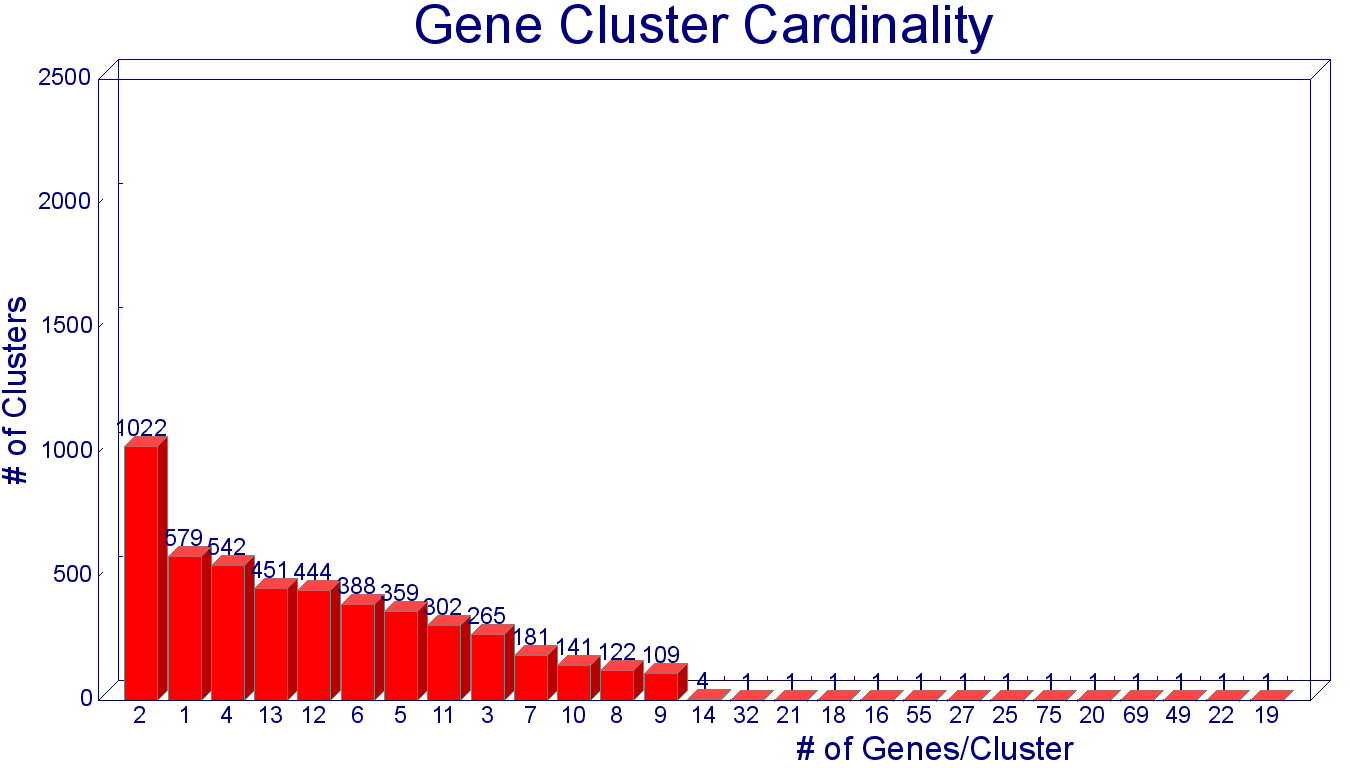
\includegraphics[width=145mm]{i75_a90_graph.png}
  
  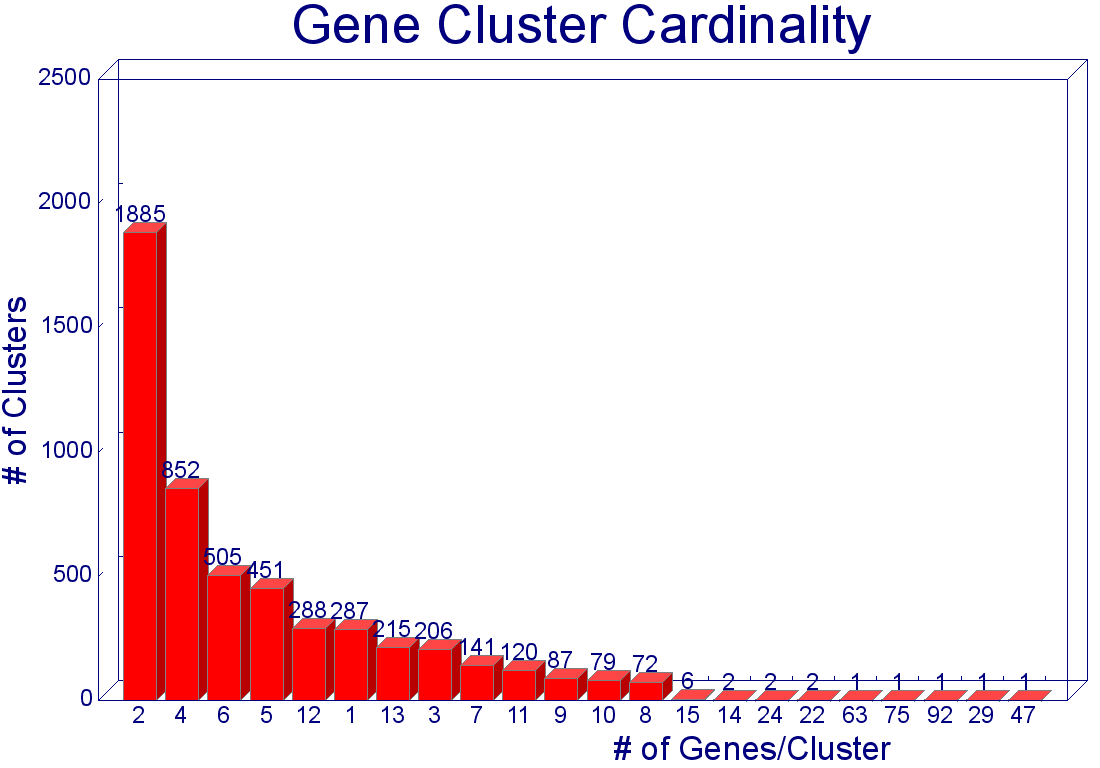
\includegraphics[width=145mm]{i90_a50_graph.png}
  
  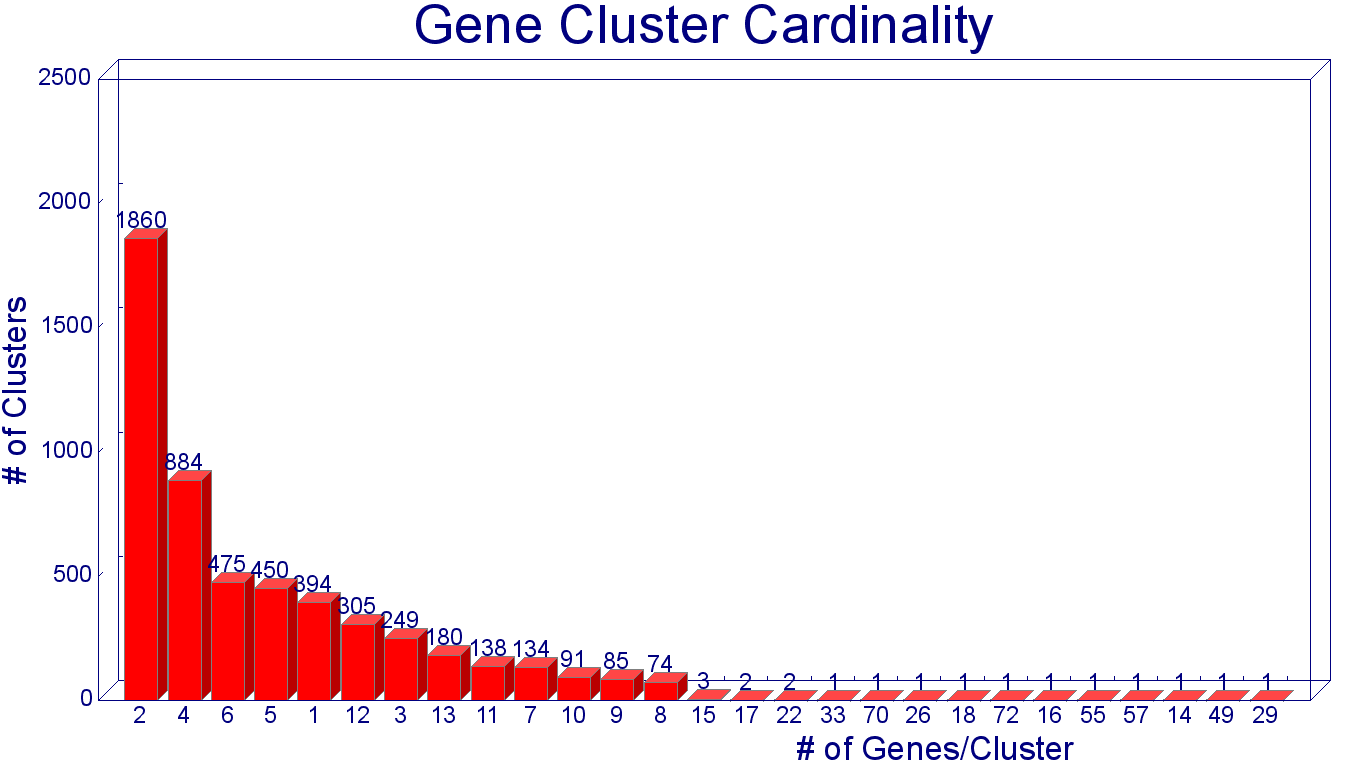
\includegraphics[width=145mm]{i90_a70_graph.png}
  
  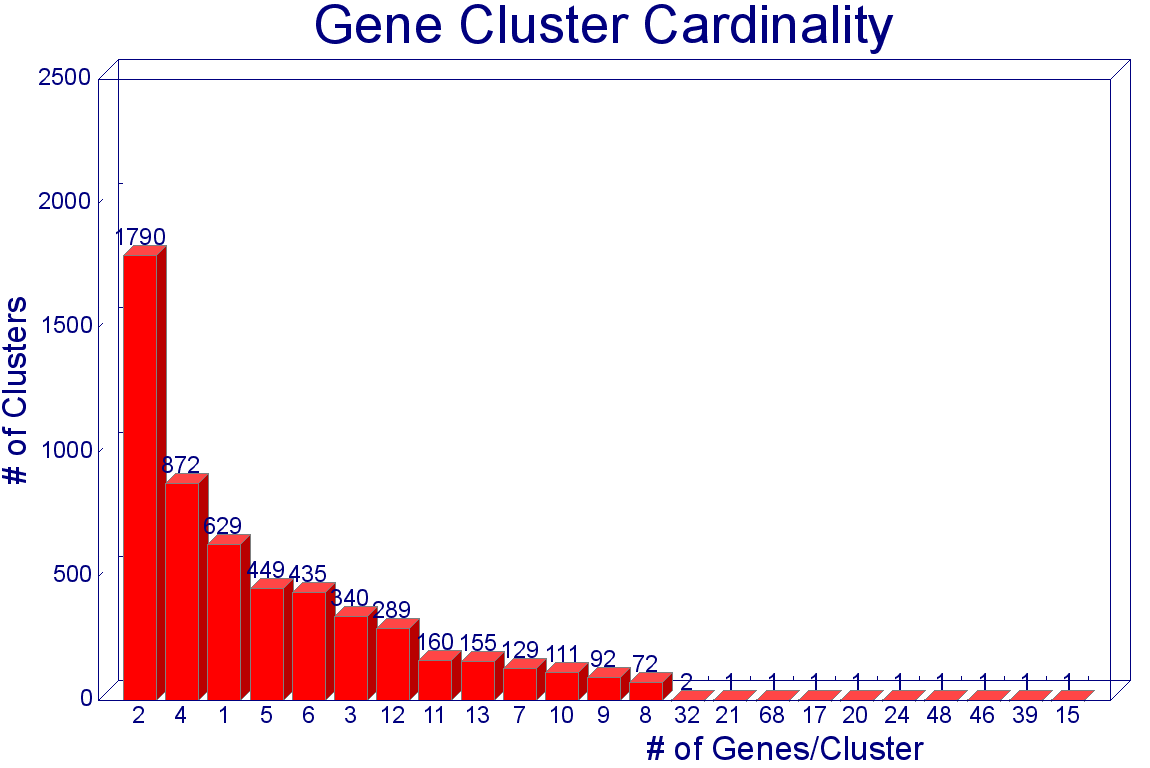
\includegraphics[width=145mm]{i90_a90_graph.png}



  {\setlength{\baselineskip}%
           {0.0\baselineskip}
  \section*{\hfill Classes}
  \hrulefill \par}

  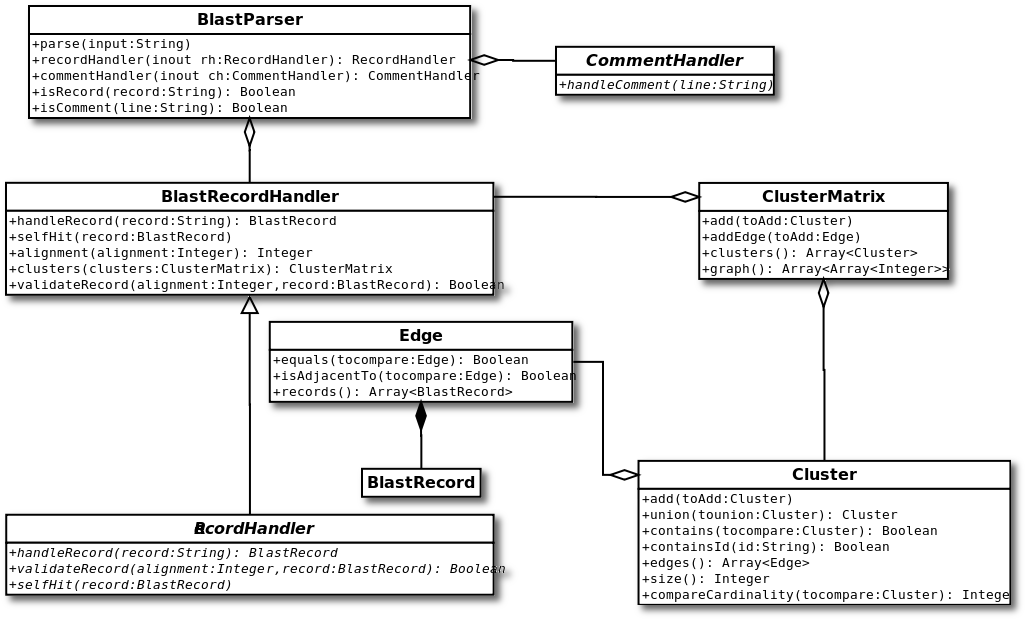
\includegraphics[width=120mm]{api/images/blast_clusters1_Class1.png}  

  
%% \tableofcontents

\section{Class \texttt{BlastParser}\label{Class_BlastParser}\index{Class BlastParser}}
\subsection*{Description\label{Description}\index{Description}}


Class mainly responsible for parsing blast input into \texttt{BlastRecord} instances.

\subsubsection*{Author: \textit{Leo Przybylski (przybyls@arizona.edu)}\label{Author:_Leo_Przybylski_przybyls_arizona_edu_}\index{Author: Leo Przybylski (przybyls@arizona.edu)}}
\subsection*{Default Constructor\label{Default_Constructor}\index{Default Constructor}}


Constructs the \texttt{BlastParser} from its attributes. A \texttt{RecordHandler} is
required. If the \texttt{CommentHandler} is not provided, a default is used.

\subsubsection*{Parameters\label{Parameters}\index{Parameters}}
\begin{description}

\item[{\texttt{rh} - a \texttt{RecordHandler} instance}] \mbox{}
\item[{\texttt{ch} - a \texttt{CommentHandler}}] \textbf{instance}\end{description}
\subsection*{Method \texttt{parse}\label{Method_parse}\index{Method parse}}


Opens the file directed by the provided filename and parses it into \texttt{BlastRecord} instances.
It then passes the \texttt{BlastRecord} instances to the \texttt{RecordHandler}

\subsubsection*{Parameters\label{Parameters}\index{Parameters}}
\begin{description}

\item[{\texttt{input} - path of the file to parse}] \mbox{}\end{description}
\subsection*{Method \texttt{parseRecord}\label{Method_parseRecord}\index{Method parseRecord}}


Takes a line from the blast output file and parses it into an array of fields

\subsubsection*{Parameters\label{Parameters}\index{Parameters}}
\begin{description}

\item[{a record from the blast output file}] \mbox{}\end{description}
\subsection*{Method \texttt{isRecord}\label{Method_isRecord}\index{Method isRecord}}


Determines if the given line is indeed a record. If it's not a record, it's probably
a comment

\subsubsection*{Parameters\label{Parameters}\index{Parameters}}
\begin{description}

\item[{a record from the blast output file}] \mbox{}\end{description}
\subsection*{Method \texttt{isComment}\label{Method_isComment}\index{Method isComment}}


Determines if the given line is indeed a comment. If it's not a comment, it's probably
a record

\subsubsection*{Parameters\label{Parameters}\index{Parameters}}
\begin{description}

\item[{a record from the blast output file}] \mbox{}\end{description}
\subsection*{Getter/Setter \texttt{commentHandler}\label{Getter_Setter_commentHandler}\index{Getter/Setter commentHandler}}


Getter/Setter for the commentHandler

\subsubsection*{Parameters\label{Parameters}\index{Parameters}}
\begin{description}

\item[{\texttt{commentHandler} to set (optional)}] \mbox{}\end{description}
\subsubsection*{Returns\label{Returns}\index{Returns}}


Gets the \texttt{commentHandler}. Only returns something if there is no parameter present.

\subsection*{Getter/Setter \texttt{recordHandler}\label{Getter_Setter_recordHandler}\index{Getter/Setter recordHandler}}


Getter/Setter for the recordHandler

\subsubsection*{Parameters\label{Parameters}\index{Parameters}}
\begin{description}

\item[{\texttt{recordHandler} to set (optional)}] \mbox{}\end{description}
\subsubsection*{Returns\label{Returns}\index{Returns}}


Gets the \texttt{recordHandler}. Only returns something if there is no parameter present.

  %% \tableofcontents

\section{Class \texttt{BlastRecordHandler}\label{Class_BlastRecordHandler}\index{Class BlastRecordHandler}}
\subsection*{Description\label{Description}\index{Description}}
\begin{verbatim}
 Allows for different types of record handling of Blast output. Used
 as an adapter passed to the BlastParser for different handling of 
 blast information.
\end{verbatim}
\subsubsection*{Author: \textit{Leo Przybylski (przybyls@arizona.edu)}\label{Author:_Leo_Przybylski_przybyls_arizona_edu_}\index{Author: Leo Przybylski (przybyls@arizona.edu)}}
\subsubsection*{Inherits From: \texttt{RecordHandler}\label{Inherits_From:_RecordHandler}\index{Inherits From: RecordHandler}}
\subsection*{Default Constructor\label{Default_Constructor}\index{Default Constructor}}


Constructs a \texttt{BlastRecordHandler} from its attributes

\subsubsection*{Parameters\label{Parameters}\index{Parameters}}
\begin{description}

\item[{a \texttt{ClusterGraph}. When it handles}] \textbf{a record, an \texttt{Gene} is added to the \texttt{ClusterGraph}. This makes the \texttt{BlastRecordHandler} stateful.}\end{description}
\subsection*{Method \texttt{handleRecord}\label{Method_handleRecord}\index{Method handleRecord}}


Creates a \texttt{BlastRecord} and handles it.

\subsubsection*{Parameters\label{Parameters}\index{Parameters}}
\begin{description}

\item[{\texttt{record} - an array of fields used}] \textbf{to populate a \texttt{BlastRecord}}\end{description}
\subsection*{Method \texttt{isSelfHit}\label{Method_isSelfHit}\index{Method isSelfHit}}


Handles \textit{self hit} blast records

\subsubsection*{Parameters\label{Parameters}\index{Parameters}}
\begin{description}

\item[{\texttt{record} - \texttt{BlastRecord} instance}] \mbox{}\end{description}
\subsection*{Getter/Setter \texttt{graph}\label{Getter_Setter_graph}\index{Getter/Setter graph}}


Getter/Setter for the cluster graph.

\subsubsection*{Parameters\label{Parameters}\index{Parameters}}
\begin{description}

\item[{\texttt{graph} to set (optional)}] \mbox{}\end{description}
\subsubsection*{Returns\label{Returns}\index{Returns}}


Gets the \texttt{graph}. Only returns something if there is no parameter present.

\subsection*{Getter/Setter \texttt{current}\label{Getter_Setter_current}\index{Getter/Setter current}}


Getter/Setter for the current cluster.

\subsubsection*{Parameters\label{Parameters}\index{Parameters}}
\begin{description}

\item[{\texttt{current} to set (optional)}] \mbox{}\end{description}
\subsubsection*{Returns\label{Returns}\index{Returns}}


Gets the \texttt{current}. Only returns something if there is no parameter present.

\subsection*{Getter/Setter \texttt{alignments}\label{Getter_Setter_alignments}\index{Getter/Setter alignments}}


Getter/Setter for the alignment length requirements hash. Each alignment length 
is stored with the query id as the key.

\subsubsection*{Parameters\label{Parameters}\index{Parameters}}
\begin{description}

\item[{\texttt{alignments} to set (optional)}] \mbox{}\end{description}
\subsubsection*{Returns\label{Returns}\index{Returns}}


Gets the \texttt{alignments}. Only returns something if there is no parameter present.

\subsection*{Method \texttt{validate}\label{Method_validate}\index{Method validate}}


Validates a \texttt{BlastRecord} or \texttt{Gene} using the self hit alignment information. If this record is valid,
we can use that information to determine if it is an gene or not.



A valid \texttt{BlastRecord} has a \% \texttt{identity} larger than that of the requirement. The \% \texttt{identity}
requirement is determined at the point when the \texttt{ClusterGraph} instance is created. That is, 
the \texttt{ClusterGraph} knows what the requirement is. The same goes for the \texttt{alignment} ratio
requirement. The \texttt{ClusterGraph} also knows what that is. The \texttt{alignment} ratio is determined by
the record alignment/self hit alignment. In order to obtain the self hit for a given record,
it is regarded that the \texttt{Cluster} the \texttt{BlastRecord} belongs in has an \texttt{Gene} somewhere with
a subject that is the same as the \texttt{BlastRecord}'s query which would make its query and subject
the same (a self hit.)



Take note that this only works if the \texttt{Cluster} that the \texttt{BlastRecord} belongs to has
a self hit. If there isn't one, then we just say it's valid. When the self hit is discovered,
this \texttt{BlastRecord} will be re-evaluated.

\subsubsection*{Parameters\label{Parameters}\index{Parameters}}
\begin{description}

\item[{\texttt{record} - The \texttt{BlastRecord}}] \textbf{or \texttt{Gene} to validate}\end{description}
\subsubsection*{Returns\label{Returns}\index{Returns}}


\texttt{1} if the record is valid, \texttt{0} otherwise.

\subsection*{Method \texttt{clusterForRecord}\label{Method_clusterForRecord}\index{Method clusterForRecord}}


Lookup the \texttt{Cluster} belonging to a \texttt{BlastRecord}. Uses both \texttt{query} and \texttt{subject}
properties of the \texttt{BlastRecord}

\subsubsection*{Parameters\label{Parameters}\index{Parameters}}
\begin{description}

\item[{\texttt{record} - The \texttt{BlastRecord}}] \textbf{or \texttt{Gene} to lookup a \texttt{Cluster} for}\end{description}
\subsubsection*{Returns\label{Returns}\index{Returns}}


A \texttt{Cluster}

  
%% \tableofcontents

\section{Class \texttt{BlastRecord}\label{Class_BlastRecord}\index{Class BlastRecord}}
\subsection*{Description\label{Description}\index{Description}}


Class representation of line items from blast output. \texttt{BlastRecord} instances 
have

\begin{description}

\item[{query id}] \mbox{}
\item[{subject id}] \mbox{}
\item[{identity}] \mbox{}
\item[{alignment length}] \mbox{}\end{description}
\subsubsection*{Author: \textit{Leo Przybylski (przybyls@arizona.edu)}\label{Author:_Leo_Przybylski_przybyls_arizona_edu_}\index{Author: Leo Przybylski (przybyls@arizona.edu)}}
\subsection*{Default Constructor\label{Default_Constructor}\index{Default Constructor}}


Constructs the \texttt{BlastRecord} from its attributes. None are required though.

\subsubsection*{Parameters\label{Parameters}\index{Parameters}}
\begin{description}

\item[{\texttt{query} id}] \mbox{}
\item[{\texttt{subject} id}] \mbox{}
\item[{\texttt{identity}}] \mbox{}
\item[{\texttt{alignment} length}] \mbox{}
\item[{\texttt{mismatches} - undetermined}] \mbox{}
\item[{\texttt{qstart} - undetermined}] \mbox{}
\item[{\texttt{qend} - undetermined}] \mbox{}
\item[{\texttt{sstart} - undetermined}] \mbox{}
\item[{\texttt{send} - undetermined}] \mbox{}
\item[{\texttt{evalue} - undetermined}] \mbox{}\end{description}
\subsection*{Method \texttt{isSelfHit}\label{Method_isSelfHit}\index{Method isSelfHit}}


A Record is considered a \textit{self hit} if its query and subject are the same. This
method compares them and returns the results. It's case-sensitive.

\subsubsection*{Returns\label{Returns}\index{Returns}}


\texttt{1} if is \textit{self hit}; otherwise, returns \texttt{0}

\subsection*{Getter/Setter \texttt{query}\label{Getter_Setter_query}\index{Getter/Setter query}}


Getter/Setter for the query

\subsubsection*{Parameters\label{Parameters}\index{Parameters}}
\begin{description}

\item[{\texttt{query\_id} to set (optional)}] \mbox{}\end{description}
\subsubsection*{Returns\label{Returns}\index{Returns}}


Gets the \texttt{query\_id}. Only returns something if there is no parameter present.

\subsection*{Getter/Setter \texttt{subject}\label{Getter_Setter_subject}\index{Getter/Setter subject}}


Getter/Setter for the subject

\subsubsection*{Parameters\label{Parameters}\index{Parameters}}
\begin{description}

\item[{\texttt{subject\_id} to set (optional)}] \mbox{}\end{description}
\subsubsection*{Returns\label{Returns}\index{Returns}}


Gets the \texttt{subject\_id}. Only returns something if there is no parameter present.

\subsection*{Getter/Setter \texttt{identity}\label{Getter_Setter_identity}\index{Getter/Setter identity}}


Getter/Setter for the identity

\subsubsection*{Parameters\label{Parameters}\index{Parameters}}
\begin{description}

\item[{\texttt{identity} to set (optional)}] \mbox{}\end{description}
\subsubsection*{Returns\label{Returns}\index{Returns}}


Gets the \texttt{identity}. Only returns something if there is no parameter present.

\subsection*{Getter/Setter \texttt{alignment}\label{Getter_Setter_alignment}\index{Getter/Setter alignment}}


Getter/Setter for the alignment

\subsubsection*{Parameters\label{Parameters}\index{Parameters}}
\begin{description}

\item[{\texttt{alignment} to set (optional)}] \mbox{}\end{description}
\subsubsection*{Returns\label{Returns}\index{Returns}}


Gets the alignment. Only returns something if there is no parameter present.

\subsection*{Getter/Setter \texttt{mismatches}\label{Getter_Setter_mismatches}\index{Getter/Setter mismatches}}


Getter/Setter for the mismatches

\subsubsection*{Parameters\label{Parameters}\index{Parameters}}
\begin{description}

\item[{\texttt{mismatches} to set (optional)}] \mbox{}\end{description}
\subsubsection*{Returns\label{Returns}\index{Returns}}


Gets the mismatches. Only returns something if there is no parameter present.

\subsection*{Getter/Setter \texttt{qstart}\label{Getter_Setter_qstart}\index{Getter/Setter qstart}}


Getter/Setter for the qstart

\subsubsection*{Parameters\label{Parameters}\index{Parameters}}
\begin{description}

\item[{\texttt{qstart} to set (optional)}] \mbox{}\end{description}
\subsubsection*{Returns\label{Returns}\index{Returns}}


Gets the qstart. Only returns something if there is no parameter present.

\subsection*{Getter/Setter \texttt{qend}\label{Getter_Setter_qend}\index{Getter/Setter qend}}


Getter/Setter for the qend

\subsubsection*{Parameters\label{Parameters}\index{Parameters}}
\begin{description}

\item[{\texttt{qend} to set (optional)}] \mbox{}\end{description}
\subsubsection*{Returns\label{Returns}\index{Returns}}


Gets the qend. Only returns something if there is no parameter present.

\subsection*{Getter/Setter \texttt{sstart}\label{Getter_Setter_sstart}\index{Getter/Setter sstart}}


Getter/Setter for the sstart

\subsubsection*{Parameters\label{Parameters}\index{Parameters}}
\begin{description}

\item[{\texttt{sstart} to set (optional)}] \mbox{}\end{description}
\subsubsection*{Returns\label{Returns}\index{Returns}}


Gets the sstart. Only returns something if there is no parameter present.

\subsection*{Getter/Setter \texttt{send}\label{Getter_Setter_send}\index{Getter/Setter send}}


Getter/Setter for the send

\subsubsection*{Parameters\label{Parameters}\index{Parameters}}
\begin{description}

\item[{\texttt{send} to set (optional)}] \mbox{}\end{description}
\subsubsection*{Returns\label{Returns}\index{Returns}}


Gets the send. Only returns something if there is no parameter present.

\subsection*{Getter/Setter \texttt{evalue}\label{Getter_Setter_evalue}\index{Getter/Setter evalue}}


Getter/Setter for the evalue

\subsubsection*{Parameters\label{Parameters}\index{Parameters}}
\begin{description}

\item[{\texttt{evalue} to set (optional)}] \mbox{}\end{description}
\subsubsection*{Returns\label{Returns}\index{Returns}}


Gets the evalue. Only returns something if there is no parameter present.

  \include{api/ClusterMatrix}
  %% \tableofcontents

\section{Class \texttt{Cluster}\label{Class_Cluster}\index{Class Cluster}}
\subsection*{Description\label{Description}\index{Description}}


A cluster is basically like a set genes in a digraph of genes where 
adjacent genes are grouped together. One Gene is known to be adjacent 
to another gene if its query points to the subject or query of another
or its subject points to the query or subject of another.
...



Being that a Cluster is a Set, there is no duplication

\subsubsection*{Author: \textit{Leo Przybylski (przybyls@arizona.edu)}\label{Author:_Leo_Przybylski_przybyls_arizona_edu_}\index{Author: Leo Przybylski (przybyls@arizona.edu)}}
\subsection*{Method \texttt{add}\label{Method_add}\index{Method add}}


Adds an \texttt{Gene} instance to the \texttt{Cluster}

\subsubsection*{Parameters\label{Parameters}\index{Parameters}}
\begin{description}

\item[{\texttt{toadd} - \texttt{Gene} instance}] \textbf{to add}\end{description}
\subsection*{Method \texttt{union}\label{Method_union}\index{Method union}}


Unions this \texttt{Cluster} instance with another \texttt{Cluster} instance. The result
is a completely new \texttt{Cluster}.

\subsubsection*{Parameters\label{Parameters}\index{Parameters}}
\begin{description}

\item[{\texttt{other} - a \texttt{Cluster} instance}] \textbf{to union with this}\end{description}
\subsubsection*{Returns\label{Returns}\index{Returns}}


A new \texttt{Cluster} instance containing all \texttt{Gene} instances from both \texttt{Cluster} instances. If 
a union is not possible, nothing is returned

\subsection*{Method \texttt{contains}\label{Method_contains}\index{Method contains}}


Traverses the \texttt{Cluster} for a given \texttt{Gene}

\subsubsection*{Parameters\label{Parameters}\index{Parameters}}
\begin{description}

\item[{\texttt{tocompare} - \texttt{Gene} to test}] \textbf{for existence}\end{description}
\subsubsection*{Returns\label{Returns}\index{Returns}}


\texttt{1} if \texttt{\$tocompare} is contained in the \texttt{Cluster}; \texttt{0} otherwise.

\subsection*{Method \texttt{indexOf}\label{Method_indexOf}\index{Method indexOf}}


Traverses the \texttt{Cluster} looking for the array index of the \texttt{Gene}

\subsubsection*{Parameters\label{Parameters}\index{Parameters}}
\begin{description}

\item[{\texttt{tocompare} - \texttt{Gene} to find}] \mbox{}\end{description}
\subsubsection*{Returns\label{Returns}\index{Returns}}


\texttt{index} integer location of \texttt{\$tocompare} within the \texttt{Cluster} array of \texttt{Gene} instances; \texttt{-1} otherwise.

\subsection*{Method \texttt{remove}\label{Method_remove}\index{Method remove}}


Locates and removes an \texttt{Gene} from the \texttt{Cluster}. This probably only happens
when an \texttt{Gene} has been found to be invalid.

\subsubsection*{Parameters\label{Parameters}\index{Parameters}}
\begin{description}

\item[{\texttt{tocompare} - \texttt{Gene} to locate}] \textbf{and remove}\end{description}
\subsection*{Method \texttt{containsId}\label{Method_containsId}\index{Method containsId}}
\subsubsection*{Parameters\label{Parameters}\index{Parameters}}
\begin{description}

\item[{\texttt{tocompare} -}] \mbox{}\end{description}
\subsubsection*{Returns\label{Returns}\index{Returns}}


\texttt{1} if \texttt{\$tocompare} is contained in the \texttt{Cluster}; \texttt{0} otherwise.

\subsection*{Getter \texttt{graph}\label{Getter_graph}\index{Getter graph}}
\subsubsection*{Returns\label{Returns}\index{Returns}}


A reference to an array instance containing \texttt{Gene} instances for this \texttt{Cluster}

\subsection*{Getter \texttt{genes}\label{Getter_genes}\index{Getter genes}}
\subsubsection*{Returns\label{Returns}\index{Returns}}


A reference to an array instance containing \texttt{Gene} instances for this \texttt{Cluster}

\subsection*{Getter \texttt{ids}\label{Getter_ids}\index{Getter ids}}
\subsubsection*{Returns\label{Returns}\index{Returns}}


A reference to an array instance containing \texttt{Gene} instances for this \texttt{Cluster}

\subsection*{Getter \texttt{size}\label{Getter_size}\index{Getter size}}
\subsubsection*{Returns\label{Returns}\index{Returns}}


The number of \texttt{Gene} instances that are part of this \texttt{Cluster}

\subsection*{Method \texttt{hasAdjacentGene}\label{Method_hasAdjacentGene}\index{Method hasAdjacentGene}}


Compares this \texttt{Cluster} to another to see if the two might have genes that 
are adjacent to each other

\subsubsection*{Parameters\label{Parameters}\index{Parameters}}
\begin{description}

\item[{\texttt{tocompare} - a \texttt{Cluster}}] \textbf{whose \texttt{Gene} instances to compare to this one for adjacency}\end{description}
\subsubsection*{Returns\label{Returns}\index{Returns}}


\texttt{1} if \texttt{tocompare} shares at least 1 adjacent gene with this \texttt{Cluster} instance or
\texttt{0} if it doesn't.

\subsection*{Method \texttt{hasGeneAdjacentTo}\label{Method_hasGeneAdjacentTo}\index{Method hasGeneAdjacentTo}}


Compares \texttt{Gene} instances in this \texttt{Cluster} to another to see if the the other 
is adjacent to any \texttt{Gene} instances in this cluster.

\subsubsection*{Parameters\label{Parameters}\index{Parameters}}
\begin{description}

\item[{\texttt{tocompare} - a \texttt{Gene} who}] \textbf{compare to others in this \texttt{Cluster} for adjacency}\end{description}
\subsubsection*{Returns\label{Returns}\index{Returns}}


\texttt{1} if \texttt{tocompare} shares at least 1 adjacent gene with this \texttt{Cluster} instance or
\texttt{0} if it doesn't.

\subsection*{Method \texttt{compareCardinality}\label{Method_compareCardinality}\index{Method compareCardinality}}


Compares the cardinality (the number of \texttt{Gene} instances) of this \texttt{Cluster} instance
to another \texttt{Cluster} instance.

\subsubsection*{Parameters\label{Parameters}\index{Parameters}}
\begin{description}

\item[{\texttt{tocompare} - a \texttt{Cluster}}] \textbf{instance to compare this against}\end{description}
\subsubsection*{Returns\label{Returns}\index{Returns}}
\begin{description}

\item[{\texttt{-1} if this \texttt{Cluster} is}] \textbf{smaller in cardinality than \texttt{tocompare}}
\item[{\texttt{0} if this \texttt{Cluster} is shares}] \textbf{the same cardinality as \texttt{tocompare}}
\item[{\texttt{1} if this \texttt{Cluster} is larger}] \textbf{in cardinality than \texttt{tocompare}}\end{description}
\subsection*{Getter \texttt{geneByHit}\label{Getter_geneByHit}\index{Getter geneByHit}}


Gets an \texttt{Gene} from the graph by the subject id. It will iterate through
the genes until it finds one with the subject id it's looking for.

\subsubsection*{Parameters\label{Parameters}\index{Parameters}}
\begin{description}

\item[{\texttt{subject} id of the \texttt{Gene}}] \textbf{to find}\end{description}
\subsubsection*{Returns\label{Returns}\index{Returns}}


An \texttt{Gene} instance

  %% \tableofcontents

\section{Class \texttt{CommentHandler}\label{Class_CommentHandler}\index{Class CommentHandler}}
\subsection*{Description\label{Description}\index{Description}}


An interface for handling comments in blast output.

\subsubsection*{Author: \textit{Leo Przybylski (przybyls@arizona.edu)}\label{Author:_Leo_Przybylski_przybyls_arizona_edu_}\index{Author: Leo Przybylski (przybyls@arizona.edu)}}
\subsection*{Default Constructor\label{Default_Constructor}\index{Default Constructor}}


Constructs the \texttt{CommentHandler} from its attributes. None are required though.

\subsection*{Method \texttt{handleComment}\label{Method_handleComment}\index{Method handleComment}}


Stub method for handling comments. This is the method that the \texttt{BlastParser} will call
when it encounters a comment.

  \include{api/Edge}
  
\section{Class \texttt{RecordHandler}\label{Class_RecordHandler}\index{Class RecordHandler}}
\subsection*{Description\label{Description}\index{Description}}


Abstract class for creating instances used by the BlastParser for handling
records.

\subsubsection*{Author: \textit{Leo Przybylski (przybyls@arizona.edu)}\label{Author:_Leo_Przybylski_przybyls_arizona_edu_}\index{Author: Leo Przybylski (przybyls@arizona.edu)}}
\subsection*{Default Constructor\label{Default_Constructor}\index{Default Constructor}}


Constructs the \texttt{RecordHandler} from its attributes. None are required though.

\subsection*{Method \texttt{handleRecord}\label{Method_handleRecord}\index{Method handleRecord}}


Stub method for handling blast output records. This is the method that the 
\texttt{BlastParser} will call when it encounters a record.

\subsection*{Method \texttt{handleRecord}\label{Method_handleRecord}\index{Method handleRecord}}


Stub method for validating blast output records. Typically, the result will
be an \texttt{Edge} added to a \texttt{Cluster}


\end{document}

